\chapter{Light Propagation in Linear Anisotropic Dielectrics}
\textit{"C'est mon chapitre préféré, celui que j'ai choisi lorsque j'étais à votre place. Ne ne négligez pas!}

\section{Anisotropic Materials in Photonics}
Beaucoup de matériaux ont des propriétés optiques quid épendent de la direction de la lumière ou de sa polarisation. 
Notons que dans un polariseur, si les polymères sont étendus en $y$, l'onde qui passera sera en $x$ !

\section{The Susceptibility and Dielectric Tensors}
\subsection{Constitutive Equations in Anisotropic Media}
	\begin{wrapfigure}[8]{l}{8cm}
	%\vspace{-5mm}
	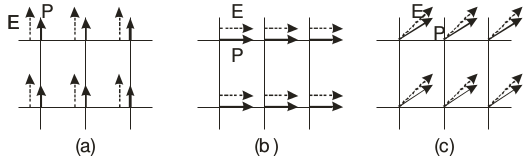
\includegraphics[scale=0.4]{ch4/image1.png}
	\captionof{figure}{ }
	\end{wrapfigure}
Lorsque le matériau n'est pas isotrope, $\vec{P}$ n'est pas toujours parallèle à $\vec{E}$ : la polarisation va
dépendre de la direction du champ électrique. Si dans une direction nous avons $n_1$ et dans une autre $n_2$ 
avec $n_a<n_b$, la superposition des deux donnera une polarisation non parallèle au champ appliqué. \\

La relation linéaire la plus générale entre deux vecteurs est un tenseur du second rang. Dès lors
\begin{equation}
P = \epsilon_0\overline{\overline{\chi}}E\qquad\text{ou}\qquad P_i = \epsilon_0\chi_{ij}E_j
\end{equation}
où $\overline{\overline{\chi}}$ est le \textbf{tenseur de susceptibilité}. S'il est diagonal avec tout des 
coefficients identiques, on se retrouve au cas du chapitre 2. Mais si non, la polarisation induite peut dépendre
de la direction de $\vec{E}$.

\subsection{Symmetry of the Susceptibility Tensor}
Il est simple de montrer analytiquement que le tenseur de susceptibilité est symétrique (sous certaines conditions).
Soit le théorème de Poynting
\begin{equation}
\dfrac{\partial U}{\partial t} = -\nabla.S-EJ_p
\end{equation}
où $U$ est la densité d'énergie EM et $\vec{S}$ le vecteur de Poynting
\begin{equation}
U = \frac{1}{2}\epsilon_0\left(|E|^2-c^2|B|^2\right),\qquad\qquad
S \equiv \left\langle \vec{E}\times\vec{H}\right\rangle = \frac{1}{\mu_0}
\left\langle \vec{E}\times\vec{B}\right\rangle
\end{equation}
Comme il  n'y a pas de courants libre, de magnétisation, le milieu est transparent et non-dissipant, l'énergie
n'est pas convertie en chaleur. L'énergie du champ peut aller dans la matière, mais elle sera "rendue" au final.
Il doit donc être possible de noter le troisième terme sous la forme d'une dérivée temporelle ou d'une divergence
afin de la faire passer dans le membre de gauche.\\

Dans la convention d'Einstein
\begin{equation}
E_kJ_{p,k} = E_k\frac{\partial P_k}{\partial t} = \frac{1}{2}E_k\epsilon_0\chi_{kl}\frac{\partial E_l}{\partial t}+
\frac{1}{2}E_l\epsilon_0\chi_{lk}\frac{\partial E_k}{\partial t}
\end{equation}
On peut toujours écrire $\chi_{kl} = \chi_{kl}^S+\chi_{kl}^A$. Il nous faudra montrer que $\chi_{kl}^A$ est
nulle. Le terme source devient\footnote{Voir page 62 pour le détail}
\begin{equation}
E_kJ_{p,k} = \frac{1}{2}\epsilon_0\chi_{kl}^S\frac{\partial (E_kE_l)}{\partial t}+\frac{1}{2}
\epsilon_0\chi_{kl}^A\left(E_k\frac{\partial E_l}{\partial t}-E_l\frac{\partial E_k}{\partial t}\right)
\end{equation}
Seule la partie symétrique peut s'écrire sous la forme d'une dérivée temporelle, la partie antisymétrique doit
forcément être nulle. Poynting s'écrit alors
\begin{equation}
\dfrac{\partial U_{total}}{\partial t}= -\nabla S
\end{equation}
où $U_{total}$ est la densité d'énergie totale
\begin{equation}
U_{total} = \frac{1}{2}D.E+\frac{1}{2}B.H
\end{equation}
Ceci n'est vrai que pour les matériaux non magnétique et non-dispersif.


\section{Plane Monochromatic Waves in Anisotropic Media}
\subsection{Dispersion Relation}
Nous allons ici analyser sir les ondes planes monochromatiques sont toujours solutions des équations de 
Maxwell et des équations constitutives (soit les équations de l’électrodynamique). Nous avons\footnote{Détails
page 63}
\begin{equation}
\nabla\times\left(\nabla\times\vec{E}\right) = -\frac{1}{c^2}\dfrac{\overline{\overline{\epsilon}}}{\epsilon_0}
\frac{\partial^2E}{\partial t^2}
\label{eq:4.41}
\end{equation}
C'est difficile, mais il existe un système de coordonnées ou ce tenseur est diagonal : tout va devenir "simple"
\footnote{Résultat attendu : le tenseur $\epsilon$ doit être symétrique, il doit exister une base où il est
diagonal}. Dans un tel système, le tenseur diélectrique est donné par (semble trivial, mais en réalité profond)
\begin{equation}
\dfrac{\overline{\overline{\epsilon}}}{\epsilon_0} =\left(\begin{array}{ccc}
n_1^2 & 0 &0\\
0 &n_2^2 &0\\
0&0&n_3^2
\end{array}\right)
\end{equation}
où $n_i$ sont les indices de réfraction principaux. L'équation \eqref{eq:4.41} devient quelque chose de 
"\textit{pas si moche}" : 
\begin{equation}
\vec\nabla\times(\vec\nabla\times\vec E) = -\frac{1}{c^2}\left(\vec{1_x} n_1^2\dfrac{\partial^2 E_x}{\partial t^2}
+\vec{1_y} n_2^2\dfrac{\partial^2 E_y}{\partial t^2}+\vec{1_z} n_3^2\dfrac{\partial^2 E_z}{\partial t^2}\right)
\end{equation}
On veut trouver une relation de dispersion $\omega(k)$. On propose une solution d'onde plane monochromatique 
de pulsation $\omega$ et de vecteur d'onde $\vec{k}$ à cette équation différentielle
\begin{equation}
E = E_0e^{i(\omega t-k.r)}
\end{equation}
En substituant cet ansat, on trouve (rot $\to\ ik$)
\begin{equation}
i\vec k\times(i\vec k\times \vec E_0) = \frac{\omega^2}{c^2}\left(\vec 1_x n_1^ 2 E_{0x}+
\vec 1_y n_2^ 2 E_{0y}+\vec 1_z n_3^ 2 E_{0z}\right)
\end{equation}
Sachant que $\vec A\times(\vec B\times \vec C) = -(\vec A\vec B)\vec C+(\vec A\vec C)\vec B$ 
\begin{equation}
\vec k(\vec k . \vec E_0) - \vec E_0 k^2 = -\frac{\omega^2}{c^2}\left(\vec 1_x n_1^ 2 E_{0x}+
\vec 1_y n_2^ 2 E_{0y}+\vec 1_z n_3^ 2 E_{0z}\right)
\end{equation}
Il s'agit de la relation de dispersion pour un milieu linéaire non isentropique. En projetant cette équation 
sur les axes principaux (par exemple sur $\vec 1_x$ on a : $k_x \vec 1_x \left(k_x E_{0x} + k_y E_{0y} + k_z E_{0z}\right) - E_{0x} \vec 1_x\left(k_xk_x + k_y k_y + k_z k_z\right) =
-\frac{\omega^2}{c^2} \vec 1_x n_1^2 E_{0x}$) on voit que la relation de dispersion est un système linéaire
en les trois composantes du champ électrique
\begin{equation}
\left(\begin{array}{ccc}
\frac{\omega^2}{c^2}n_1^2-k_y^2k_z^2 & k_xk_y & k_xk_z\\
k_yk_x & \frac{\omega^2}{c^2}n_2^2-k_x^2-k_z^2 & k_yk_z\\
k_zk_x & k_zk_y & \frac{\omega^2}{c^2}n_3^2-k_x^2-k_y^2
\end{array}\right)\left(\begin{array}{c}
E_{0x}\\
E_{0y}\\
E_{0z}
\end{array}\right) = 0
\label{eq:4.19}
\end{equation}



\subsection{The Normal Surface}
Considérons d'abord quelques situations simplifiées
\begin{enumerate}
\item Vecteur d'onde parallèle à $\vec{1_x}$ : $k_x=k$. Le système \eqref{eq:4.19} se réduit à 
\begin{equation}
\left\{\begin{array}{rl}
\DS\frac{\omega^ 2}{c^2}n_1^2 E_{0x} &= 0\vspace{2mm}\\
\DS\left(\frac{\omega^2}{c^2}n_2^2-k^2\right)E_{0y}&=0\vspace{2mm}\\
\DS\left(\frac{\omega^2}{c^2}n_3^2-k^2\right)E_{0z}&=0
\end{array}\right.
\end{equation}
La première équation nous informe que le champ est transverse et les deux dernières les solutions : si les $E_{0i}$
sont non-nuls, la parenthèse doit l'être : on en tire les relations de dispersions.La première est l'onde plane
polarisée selon $y$ de nombre d'onde $k_2$
\begin{equation}
E^{(1)} = \vec{1_y}E_0^{(1)}e^{i(\omega t-k_2x)}\qquad\text{ où }\quad k_2 = \frac{\omega}{c}n_2
\end{equation}
La seconde est l'onde plane polarisée selon $z$ de nombre d'onde $k_3$
\begin{equation}
E^{(2)} = \vec{1_z}E_0^{(2)}e^{i(\omega t-k_3x)}\qquad\text{ où }\quad k_3 = \frac{\omega}{c}n_3
\end{equation}
\end{enumerate}





